\section{Les types de base de Python}
\subsection{Quelques types simples}
% 1 Les types de base Python
% 1.1 Quelques types simples
%     - entiers
%     - flottants
%     - True, False
%     - None

\begin{frame}
  \frametitle{Quelques types simples}
  \begin{itemize}
    \item<1-> les entiers
    \item<2-> les flottants
    \item<3-> les booléens
    \item<4-> la valeur 'Rien'
  \end{itemize}
\end{frame}

\begin{frame}
  \frametitle{Quelques types simples}
    \begin{itemize}
      \item les entiers
    \end{itemize}
    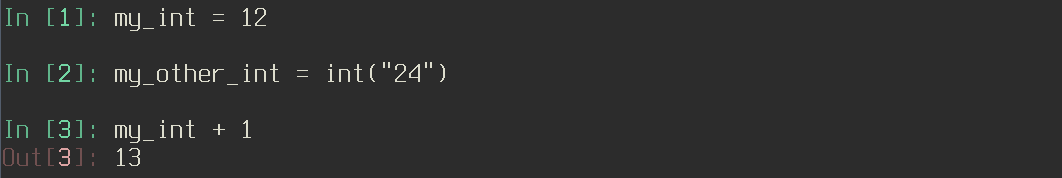
\includegraphics[scale=0.35]{type_int.png}
\end{frame}

\begin{frame}
  \frametitle{Quelques types simples}
    \begin{itemize}
      \item les flottants
    \end{itemize}
    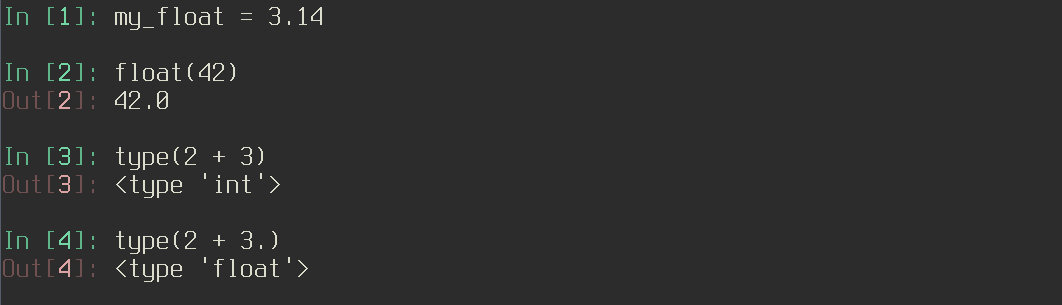
\includegraphics[scale=0.35]{type_float.png}
\end{frame}

\begin{frame}
  \frametitle{Quelques types simples}
    \begin{itemize}
      \item les booléens : \alert{True, False}
      \item la valeur 'Rien' : \alert{None}
    \end{itemize}
\end{frame}

% 1.2 Quelques structures de données
%     - les chaines de caractère sont des séquences comme les autres
%     - séquence: list modifiable, tuple non modifiable, queue...
%     - dictionnaire
%     - ensemble (partie gauche d'un dict): set modifiable, frozenset non modifiable

\subsection{Quelques structures de données}
\begin{frame}
  \frametitle{Quelques structures de données}
  \begin{itemize}
      \item<1-> les chaînes de caractère, un cas particulier de séquence
      \item<2-> les autres séquences : tuples, listes, queue, \ldots
      \item<3-> les dictionnaires
      \item<4-> les sets, frozenset
    \end{itemize}
\end{frame}

\begin{frame}
  \frametitle{Quelques structures de données}
    \begin{itemize}
      \item les chaînes de caractères
    \end{itemize}
    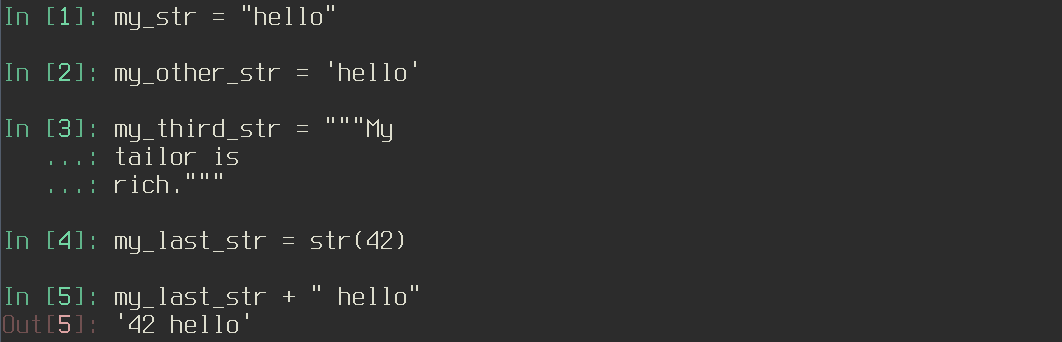
\includegraphics[scale=0.35]{type_str.png}
\end{frame}

\begin{frame}
  \frametitle{Quelques structures de données}
    \begin{itemize}
      \item les tuples
    \end{itemize}
    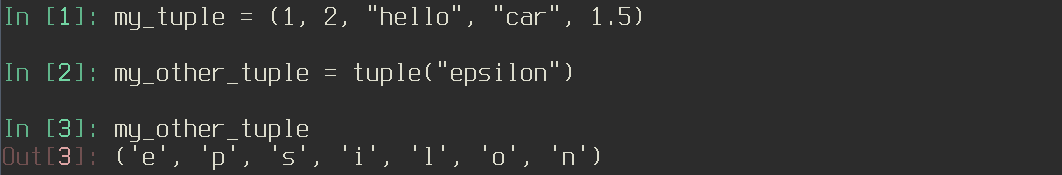
\includegraphics[scale=0.35]{type_tuple.png}
\end{frame}

\begin{frame}
  \frametitle{Quelques structures de données}
    \begin{itemize}
      \item les listes
    \end{itemize}
    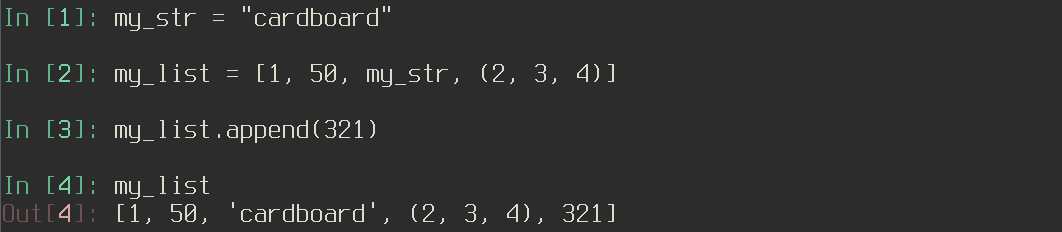
\includegraphics[scale=0.35]{type_list.png}
\end{frame}

\begin{frame}
  \frametitle{Quelques structures de données}
    \begin{itemize}
      \item les dictionnaires
    \end{itemize}
    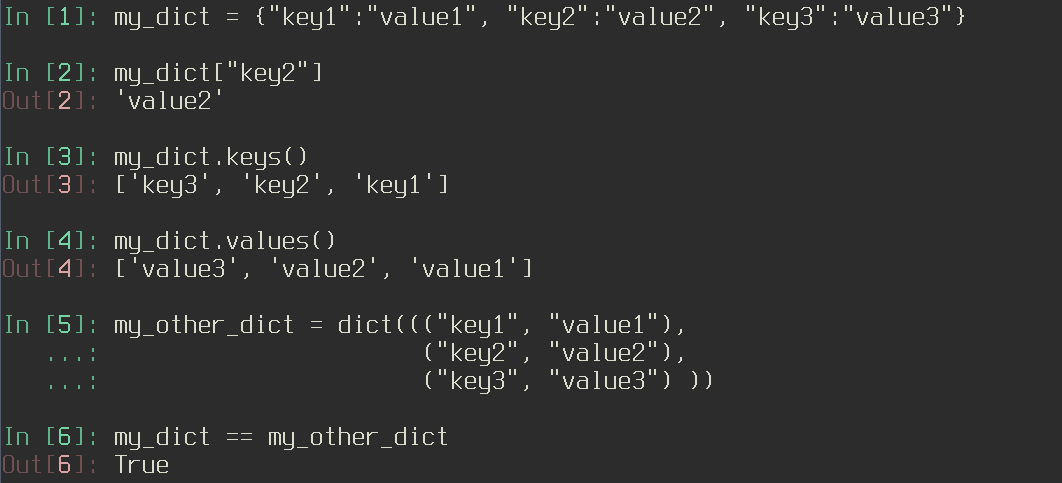
\includegraphics[scale=0.35]{type_dict.png}
\end{frame}

\begin{frame}
  \frametitle{Quelques structures de données}
    \begin{itemize}
      \item les sets
    \end{itemize}
    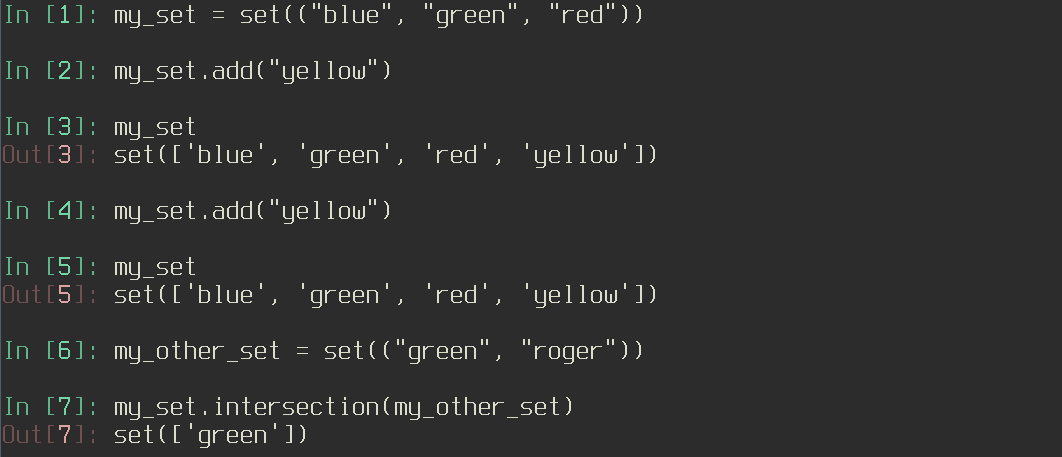
\includegraphics[scale=0.35]{type_set.png}
\end{frame}

% 1.3 Quelques autres types courants (juste les évoquer)
%     - classe, fonction ou méthode, module...

\subsection{Quelques autres types courants}
\begin{frame}
  \frametitle{Quelques autres types courants}
    \begin{itemize}
      \item les classes
      \item les fonctions/méthodes
      \item les modules
    \end{itemize}
\end{frame}

% 2 La syntaxe de Python
% 2.1 instructions
%     - séparateur d'instruction : ';' (éviter) ou '\\n'
% 2.2 blocs
%     - contexte (scope) défini par bloc
%     - blocs définis par :
%       - leur niveau d'indentation
%       - bloc de niveau inférieur suit une ligne
%         - qui commence par un mot clef (if, while, for, def, class, with)
%         - se termine par ':'
% et continuer comme julien l'a fait sur if etc.
% Ce point 2.2 est une introduction aux différents blocs qu'on va traiter ensuite.
